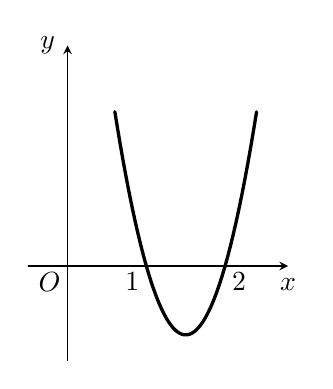
\begin{tikzpicture}[>=stealth, scale=1.0, line cap=round, line join=round]
  % Axes
  \draw[->] (-0.5, 0) -- (2.8, 0) node[below=1pt] {$x$};
  \draw[->] (0, -1.2) -- (0, 2.8) node[left=1pt] {$y$};
  \node[below left=-1pt] at (0, 0) {$O$};

  % Parabola y = 3.5*(x-1)*(x-2)
  \draw[very thick] plot[domain=0.6:2.4, samples=50] (\x, {3.5*(\x-1)*(\x-2)});

  % Ticks
  \node[below left=-1pt] at (1, 0) {$1$};
  \node[below right=-1pt] at (2, 0) {$2$};
\end{tikzpicture}
